\chapter{Background and Related Works}
The purpose of code generation tools is to help developers improve their productivity, ensure correctness of code syntax, and lessen the number of errors in software \cite{groher_01}.  The input specifications of these tools introduce additional levels of indirection to solve these problems \cite{spinellis_01}.  A range of tools have been created to generate code that can be complex and tedious to write by hand:
\begin{itemize}
  \item Scanners
  \item Parsers
  \item Interpreters
  \item Compilers
  \item Graphical user interfaces
\end{itemize}

\section{Traditional Scanner and Parser Code Generation}
The Yacc compiler-compiler \cite{johnson_01} first introduced in 1975 generates LALR parsers that must be run with a lexical analyzer generator such as Lex.  Similar to Yacc is Bison \cite{aycock_01,demaille_01}—a Yacc-compatible parser generator that accepts any properly written Yacc grammar.  Like Yacc, Bison-generated parsers read a sequence of tokens from a scanner generated by a lexical analyzer generator like Lex or flex.

\indent
To illustrate the steps of traditional parser generation using Lex and Yacc (figure ~\ref{fig:YaccGrammarRule}) \cite{johnson_01,lesk_01,niemann_01}, a file is provided by the developer containing a set of patterns that define how to separate strings found in source data.  This file is read by Lex, which uses these patterns to generate the C source code of a lexical analyzer.  This newly generated lexical analyzer uses the patterns to identify specific strings in the input and split them into tokens to simplify processing.

\begin{figure}[htbp]
\centering
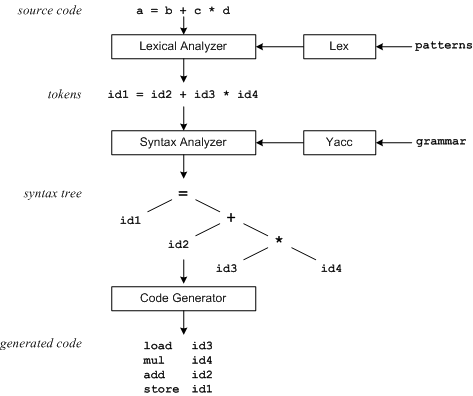
\includegraphics[width=0.9\textwidth]{figures/LexAndYaccCompileSequence.png}
\caption[Lex and Yacc Compilation Sequence]{Lex and Yacc Compilation Sequence \cite{niemann_01}}
\label{fig:LexAndYaccCompileSequence}
\end{figure}

\indent
A file containing grammar rules is provided by the developer to Yacc, which uses those rules to generate C source code for a syntax analyzer (i.e. parser).  The syntax analyzer uses this grammar to transform the tokens output by the lexical analyzer into a syntax tree.  The structure of this syntax tree implies the precedence and associativity of operators found within the tokens.  The syntax tree is then traversed in depth-first order to generate the desired source code (figure ~\ref{fig:LexAndYaccCompileSequence}) \cite{niemann_01}.

\indent
A predicated-LL(k) parser called ANTLR \cite{parr_01} was introduced by Parr and Quong in 1995.  The ANTLR parser generator was advertised to be easier to use than generators like YACC or BISON.  An LL(k) parser is a top-down parser that parses from left to right, utilizing a look-ahead of k tokens.  All parsing decisions are made solely from the next k tokens, which means that it does no backtracking.

\indent
The HYACC (Hawaii Yacc) parser generator first released in 2008 supports complete LR(0), LALR(1), LR(1), and partial LR(k) \cite{chen_01,chen_02}.  HYACC is compatible with Yacc and Bison input grammars and works with Lex.  The HYACC parser generator is notable because it can resolve reduce/reduce conflicts through its implementation of the LR(1) parser generation algorithm \cite{chen_01}.  Reduce/reduce conflicts occur when two or more rules in an input grammar apply to the same input sequence \cite{free_01}.  These conflicts are typically the result of a serious problem with an input grammar \cite{free_01}.

\begin{figure}[htbp]
\centering
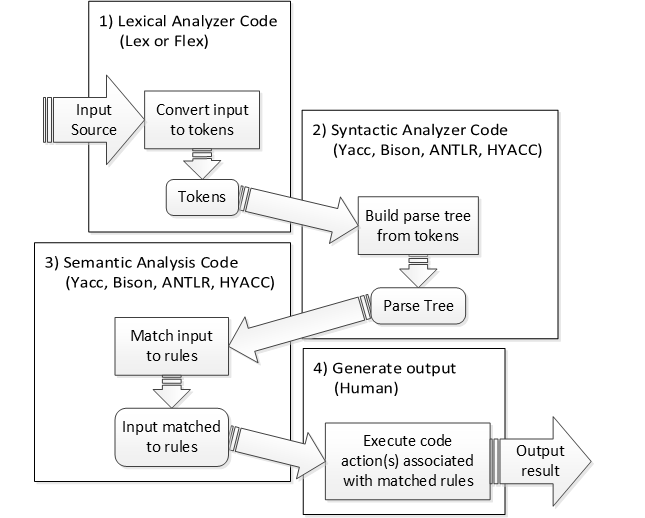
\includegraphics[width=0.9\textwidth]{figures/TraditionalCodeGenProcess.png}
\caption{Traditional code generation process using a lexical analyzer generator in conjunction with a parser generator and actions code.}
\label{fig:TraditionalCodeGenProcess}
\end{figure}

\indent
All of these parser generators provide an effective means to reduce human interaction with code (figure~\ref{fig:TraditionalCodeGenProcess}).  They have the added benefit of generating logical and syntactically correct code as long as the grammar is correct.  On the other hand, the input grammars used by these parser generators cannot be used for lexical analysis of the parser input.  Moreover, code actions that generate output are not provided as part of the input grammar.  These actions must be manually written and inserted into the code generated by the parser generator.

\section{Model-Based Parser Code Generation}

\indent
Model-based parser generators provide an alternative to traditional parser generators using a model-based language specification.  This kind of specification is explained by \cite{quesada_01} and \cite{quesada_02} as starting with an abstract syntax model (ASM) embodying the main concepts of a given language.  One or more concrete syntax models (CSMs) are created from this ASM.  Each CSM defines specific details about the language being modelled.  Elements within the ASM can then be converted into their concrete representation using a mapping of the ASM to its CSM(s).  This mapping is created by annotating the ASM with pertinent constraint metadata.  With this mapping in place, any changes to the ASM by the user will cause the language processor to automatically update to reflect those changes.

\indent
Since grammar specifications are not needed by model-based parser generators they can offer several advantages over traditional parser generators \cite{quesada_02}:
\begin{itemize}
  \item An easier language design process.  Language design is decoupled from language processing because the language grammar is automatically generated.
  \item Non-tree structures can be modeled.  This is different from traditional parser generators that force users to model a tree structure.
  \item Some semantic checks like reference resolution can be automated.
  \item Handles references between language elements, as opposed to the traditional way of resolving references manually using a symbol table.
\end{itemize}

\indent
The unique capability of model-based parser generators to use an ASM as input rather than a grammar make it possible for them to behave in two different ways \cite{quesada_02}:
\begin{enumerate}
  \item An ASM representing a tree structure (Abstract Syntax Tree) causes a model-based parser generator to behave like a traditional parser generator.
  \item An ASM representing a non-tree structure (Abstract Syntax Graph) causes a model-based parser generator to use reference resolution.
\end{enumerate} 

\indent
ModelCC is a model-based parser generator that accepts an annotated conceptual model as its input rather than a context-free grammar \cite{quesada_01}.  ModelCC uses this annotated model to generate a parser written in Java that automatically instantiates the language conceptual model \cite{quesada_01, modelcc_01}.

\indent
The process of generating a parser using ModelCC as explained by \cite{quesada_02} begins with an ASM that is defined by classes representing language elements and the relationships between them.  Metadata annotations are added to these language elements and their corresponding relationships to produce an ASM to CSM mapping.  Reference resolution is performed to match referenced objects to their equivalent object instantiations.  A parser is then generated that automatically instantiates the conceptual model.

\indent
ModelCC delivers an effective way to decrease human interaction with code by generating grammar code and lexical analysis code from an input model specification.  On the other hand, it is similar to other parser generators because it does not implicitly support specific input/output methods such as UDP/IP, etc.

